\documentclass[12pt]{article}
\usepackage{url,amsmath}
\usepackage{algorithm}
\usepackage{algpseudocode}
\usepackage{array}
\usepackage{amssymb}

\usepackage{longtable}
\usepackage{graphicx}

\renewcommand{\algorithmicrequire}{\textbf{Input:}}
\renewcommand{\algorithmicensure}{\textbf{Output:}}

\setlength{\oddsidemargin}{.25in}
\setlength{\evensidemargin}{.25in}
\setlength{\textwidth}{6.25in}
\setlength{\topmargin}{-0.4in}
\setlength{\textheight}{8.5in}

\newcommand{\heading}[5]{
   \renewcommand{\thepage}{#1-\arabic{page}}
   \noindent
   \begin{center}
   \framebox{
      \vbox{
    \hbox to 5.78in { {\bf Math/Stat 310: Intro to Mathematical Statistics}
         \hfill #2 }
       \vspace{4mm}
       \hbox to 5.78in { {\Large \hfill #5  \hfill} }
       \vspace{2mm}
       \hbox to 5.78in { {\it #3 \hfill #4} }
      }
   }
   \end{center}
%   \vspace*{4mm}
}

\newcommand{\handout}[3]{\heading{#1}{#2}{Instructor:
Hyunseung Kang}{Scribe: Meenmo Kang}{Lectures #1: #3}}

\setlength{\parindent}{0in}
\setlength{\parskip}{0.1in}

\newcommand{\Var}{{\rm Var}}
\newcommand{\E}{{\rm E}}
\newcommand{\Cov}{{\rm Cov}}
\newcommand{\Corr}{{\rm Corr}}
\newcommand{\pdf}{{\rm pdf}}
\newcommand{\mgf}{{\rm MGF}}
\newcommand{\proof}{{\bf Proof. }} %% To begin a proof write \proof
\newcommand{\qed}{\mbox{}\hspace*{\fill}\nolinebreak\mbox{$\rule{0.6em}{0.6em}$}} %%to end your proof write $\qed$.
\newcommand{\ma}{{\mathcal A}}
\newcommand{\mf}{{\mathcal F}}
\newcommand{\hs}{\heartsuit}
\newcommand{\cs}{\clubsuit}
\newcommand{\noi}{\noindent}
\newtheorem{lemma}{Lemma}
\newtheorem{theorem}[lemma]{Theorem}
\newtheorem{definition}{Definition}
\newtheorem{proposition}{Proposition}
\newtheorem{remark}{Remark}

\bibliographystyle{plain}

\begin{document}
\handout{5}{February 12, 2018}{Stratified Sampling}
%Set n to the lecture number

\begin{section}{Stratified Sampling}
When we need to collect a huge amount of data, it would be efficient to divide the data set into small groups. The small groups can be categorized by region, race, gender, or age, for example. Once the data is separated into small groups, then each of small groups is called a stratum, strata for plural. Suppose there is a large data set that was sampled in the US. The data can be categorized by 50 different states. Then the number of total strata L will be 50. After dividing up a dataset, SRS is run on each stratum.\\

\textbf{Properties of Stratified SRS}\\
Several properties of stratified SRS are denoted as shown below.\\

$n_l$: The number of people in stratum $l$ that were sampled.\\
$N_1$: Total number of people in stratum $l$.

Population: $\left\{\xi_{lk}, ... \;|\;\text{$l$ = $lth$ stratum, $k$ = $kth$ individual in stratum $l$}\right\} \Rightarrow \; N = \sum\limits_{l=1}^{L}N_l$\\
\\ 
Sample: $X_{lk} =$ 
$\begin{cases}
1\text{\quad If individual $k$ in stratum $l$ is sampled} \\
0\text{\quad Otherwise}
\end{cases}$ $\; \Rightarrow n = \sum\limits_{l=1}^{L} \sum\limits_{k=1}^{n_l} \xi_{lk} X_{lk}$\\ \newline

Joint and marginal PDF of stratified samplings are formed similarly as those of SRS, since, as I mentioned prior, SRS samplings take place after dividing up each stratum. As a result, joint and marginal PDF of stratified random samplings are denoted as follows.\\
$$pdf_l(X_{l1},X_{l2},X_{l3}, \ldots, X_{lN_l}) = \frac{1}{\binom{N_l}{n_l}} \qquad \qquad pdf(X_{lk}=1) = \frac{n_l}{N_l}$$

For stratum $l$, there are $\binom{N_l}{n_l}$ total possible ways to sample $n_l$ out of $N_l$. This means that there are $\binom{N_1}{n_1}\cdot\binom{N_2}{n_2}\ldots\binom{N_l}{n_l}$ possible stratified random samplings. Though each element of the same stratum is dependent on the other, taken by SRS, each stratum is independent. Therefore, the $pdf$ can be a product of each stratum. In mathematical notation, \\
$$pdf(X_{11},X_{12},X_{13},...,X_{lN_l}) = \prod_{l=1}^{L} pdf_l(X_{l1},X_{l2},X_{l3}, \ldots, X_{lN_l}) = \prod_{l=1}^{L} \frac{1}{\binom{N_l}{n_l}} $$\\

For example, if a data set whose N = 30,000 and n = 100 that we are working on is normally distributed, then its PDF is 
$$pdf(X_1,...,X_{100}) = \prod_{i=1}^{100} \frac{1}{\sqrt{2\pi\sigma ^2}}exp(\frac{-(X_i-\mu)^2}{2\sigma ^2})$$\\

\textbf{Population Parameters}\\
Population mean is denoted by $\mu = \frac{1}{N} \sum\limits_{l=1}^{L} \sum\limits_{k=1}^{N_l} \xi_{lk}$. Meanwhile, this can be modified using the sample mean formula as below. 
$$\mu_l = \frac{1}{N_l} \sum\limits_{k=1}^{N_l} \xi_{lk} \; \Rightarrow \;\sum\limits_{k=1}^{N_l} \xi_{lk} = \mu_l N_l \qquad \mu = \frac{1}{N} \sum\limits_{l=1}^{L} \mu_l N_l$$ 

This implies that the sum of each product of mean $\mu_l$ and the number of elements $N_l$ of stratum $l$ divided by total number of population $N$ will be population mean.\\ 

For variance, there are two different types. One is for unequal variance assumption in T test, denoted as follows.\\
$$\sigma^2 = \frac{1}{N} \sum\limits_{l=1}^{L} \sum\limits_{k=1}^{N_l} (\xi_{lk}-\mu_l)^2$$\\
For this case, each stratum has a different size of variance. As depicted below, suppose that the size of one stratum is much larger than that of another one. Then, the grand mean, which is the sum of both means divided by the total number of elements, $n_1$ and $n_2$, tends to be biased to the larger one.\\

$$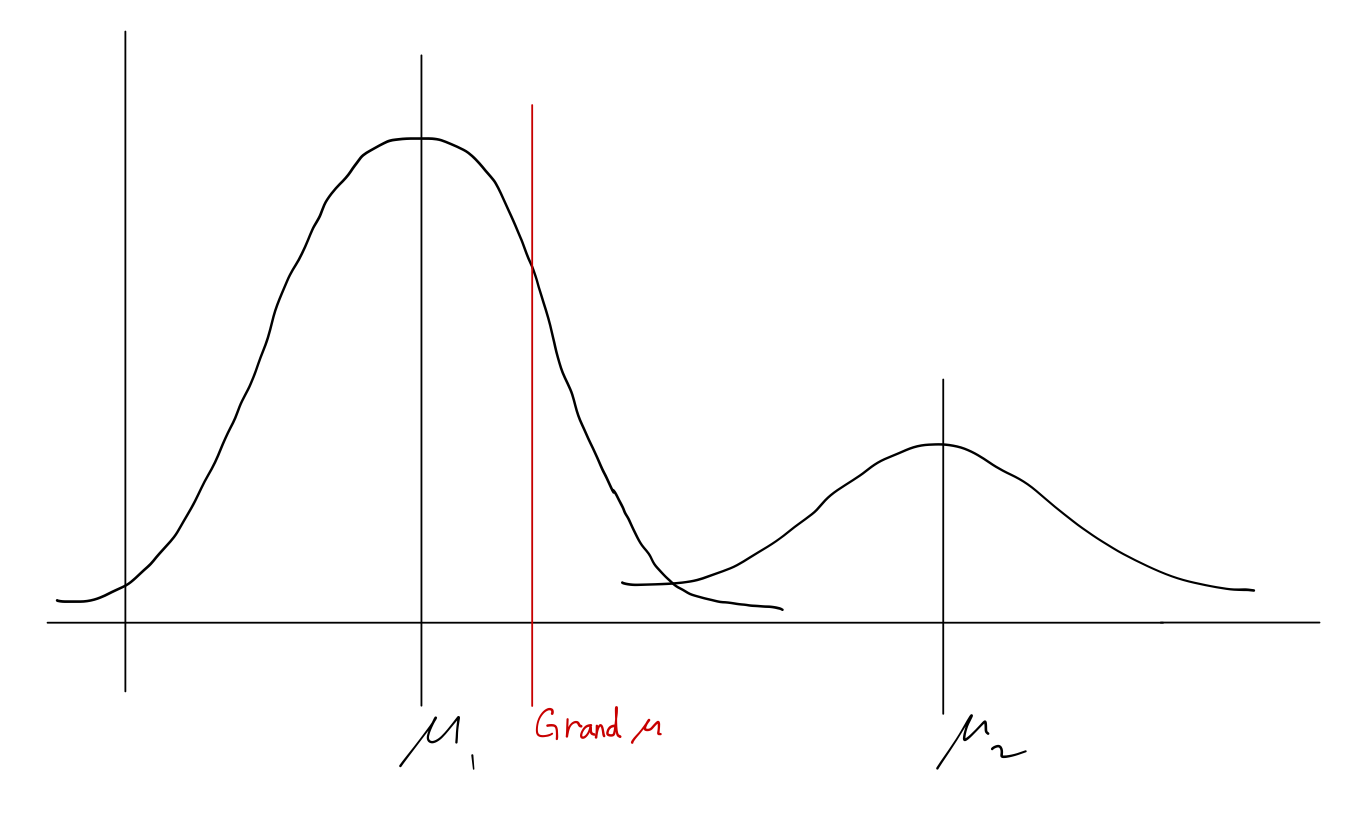
\includegraphics[height=4cm, width=8cm]{stratified_image.png}$$

Another type of variance is for pooled variance assumption, where the variance of each stratum is identical. 

$$\tilde{\sigma}^2 = \frac{1}{N} \sum\limits_{l=1}^{L} \sum\limits_{k=1}^{N_l} (\xi_{lk}-\mu)^2$$ \\
Note that $\tilde{\sigma}^2 = \sigma ^2$ if and only if $\mu = \mu_l$ for every $l$\\

\end{section}
\end{document}


